\documentclass[a4,paper,fleqn]{article}

\usepackage{layout}

\DeclareSIUnit\year{Jahr}

\title{Notizen EEV -- SW07}
\date{\today}
\author{Daniel Winz}

\begin{document}
\maketitle
\clearpage

\section{Turbinentypen}
\subsection{Freistrahlturbine}
Aktionsturbine
\begin{itemize}
    \item Pelton
\end{itemize}

\subsection{Überdruckturbine}
Reaktionsturbine
\begin{itemize}
    \item Francis
    \item Kaplan
    \item Rohr-Turbine
\end{itemize}
$\Rightarrow$ Saugrohr notwendig

\subsection{Einsatzbereich}
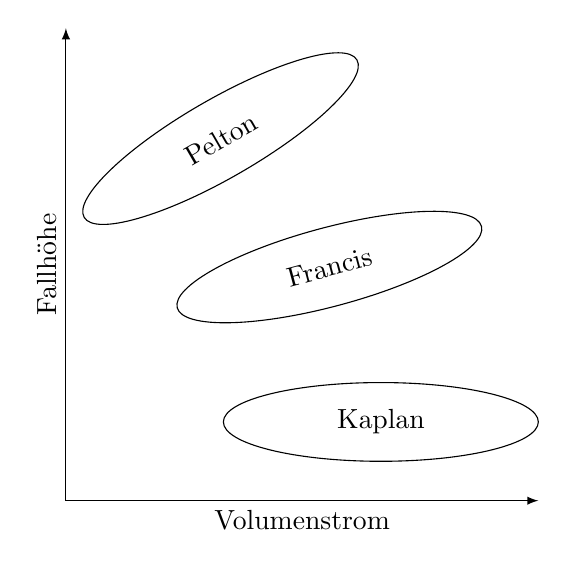
\begin{tikzpicture}
    \draw[-latex] (0,0) -- node[below] {Volumenstrom} (6,0);
    \draw[-latex] (0,0) -- node[above, rotate=90] {Fallhöhe} (0,6);
    \draw[rotate=0]  (4,1) ellipse (2 and 0.5) node[rotate=0]  {Kaplan};
    \draw[rotate=15] (4,2) ellipse (2 and 0.5) node[rotate=15] {Francis};
    \draw[rotate=30] (4,3) ellipse (2 and 0.5) node[rotate=30] {Pelton};
\end{tikzpicture}

\subsection{Wirkungsgrad}
\begin{tikzpicture}
    \draw[-latex] (0,0) -- (6,0) node[below] {Q [\si{\cubic\metre\per\second}]};
    \draw[-latex] (0,0) -- (0,6) node[left] {$\eta$};
\end{tikzpicture}

\subsection{Turbinenregelung}
\begin{itemize}
    \item Leistung\\
        Definierte Leistungsabgabe\\
        Typisch Hochdruck-Anlagen mit Speicher\\
    \item Pegel\\
        Zufluss, Stauziel konstant\\
        Typisch "'Fluss-Kraftwerk"' z.B. am Rhein
\end{itemize}

\section{Verhalten von Synchrongeneratoren am Netz}
\[ n_{syn} = \frac{60 \cdot f}{n} \]
\[ n: \text{Polpaarzahl} \]
Generator mit $n=2$: Turbo-Generator

\subsection{Leistungs-Frequenzregelung}
\begin{tikzpicture}
    \draw[-latex] (0,0) -- node[below] {Volumenstrom} (6,0);
    \draw[-latex] (0,0) -- node[above, rotate=90] {Fallhöhe} (0,6);
\end{tikzpicture}
\[ P_V: \text{Verbrauchte Wirkleistung} \]
\[ P_E: \text{Erzeugte Wirkleistung} \]
\[ \Delta P = P_E - P_V \]

\subsection{Primärregelung = Turbinenregelung}
\begin{tikzpicture}
    \draw[-latex] (0,0) -- (6,0) node[below] {f [\si{\hertz}};
    \draw[-latex] (0,0) -- (0,6) node[left] {P [\si{\kilo\watt}]};
    \draw[thick]  (0,5) -- (5,0);
    \draw[]       (0.2,2.5) -- (-0.2,2.5)  node[left]  {$f_N$};
    \draw[]       (2.5,0.2) -- (2.5,-0.2)  node[below] {$P_N$};
    \draw[dotted] (0.2,2.5) -- (2.5,2.5) -- (2.5,0.2);
    \draw[]       (0.2,2.0) -- (-0.2,2.0)  node[left]  {$f_1$};
    \draw[]       (3.0,0.2) -- (3.0,-0.2)  node[below] {$P_1$};
    \draw[dotted] (0.2,2.0) -- (3.0,2.0) -- (3.0,0.2);
    \draw[]       (0.2,3.0) -- (-0.2,3.0)  node[left]  {$f_2$};
    \draw[]       (2.0,0.2) -- (2.0,-0.2)  node[below] {$P_2$};
    \draw[dotted] (0.2,3.0) -- (2.0,3.0) -- (2.0,0.2);
\end{tikzpicture}
\\
Maschinen-Statik: 
\[ b_P = \frac{\frac{\Delta f}{f_N}}{\frac{\Delta P}{P_N}} \]
Typischer Bereich 0.01 \ldots 0.05 (1 \ldots 5 \%)
\[ b_P = \text{Statik} \Rightarrow 0.05 p.u. \text{( per Unit)} \]
Bleibender Proportionalbeiwert
\[ K_{P_b} = \frac{1}{b_P} = \frac{\frac{\Delta P}{P_N}}{\frac{\Delta f}{f_N}} \]
Leistungszahl der Maschine
\[ K_M = -\frac{\Delta P_E}{\Delta f} = \frac{100 \cdot P_N}{b_P \cdot f_N} \]


\end{document}
